\documentclass{article}
\usepackage[fleqn]{amsmath}
\usepackage{amssymb}
\usepackage{amsthm}
\usepackage{cleveref}
\usepackage{indentfirst}
\usepackage[utf8]{inputenc}
\usepackage{listings}
\usepackage{fullpage}
\usepackage{marvosym}
\usepackage{tikz}
\usepackage{tikz-qtree}
\usepackage{tipa}
\usetikzlibrary{arrows,automata}
\usepackage{wrapfig}

\crefname{section}{§}{§§}
\Crefname{section}{§}{§§}

\lstset{
numbers=left,
numberstyle=\small,
numbersep=8pt,
frame = single,
captionpos=b,
framexleftmargin=15pt}
\setlength{\belowcaptionskip}{-10pt}

\title{\vspace{5cm}Ripple \\ {\large\it make waves} \\ A Tutorial Introduction \\ Team 5}
\author{\begin{tabular}{rcl}
\textbf{Project Manager:}    &   Amar Dhingra   &   \textbf{asd2157} \\
\textbf{System Architect:}   &   Alexander Roth &   \textbf{air2112} \\
\textbf{System Integrator:}  &   Artur Renault  &   \textbf{aur2103} \\
\textbf{Language Guru:}      &   Spencer Brown  &   \textbf{stb2132} \\
\textbf{Tester \& Verifier:} &   Thomas Segarra &   \textbf{tas2172}
\end{tabular}}
\date{2015 -- 03 -- 25}

\newcommand{\code}{\texttt}
\newcommand{\back}{\textbackslash}

\begin{document}

\maketitle
\newpage
\tableofcontents
\newpage

\section{Introduction}
Our introduction to Ripple is focused on getting you, the developer, quickly up to speed with the structure and usage of Ripple. While this introduction is not as thorough as the reference manual, we hope that after reading this you will be prepared to write clean reactive programs.

Before we begin, we need to answer the question: What is Ripple? Ripple is an imperative language that implements the reactive programming paradigm. A discussion on reactive programming, along with example use cases, can be found later in this tutorial.

Ripple closely resembles code from languages in the C family, but is more focused on one specific problem than its peers; Ripple focuses on the problem of creating programs that intuitively interact with dynamic data. As such, the most important aspect of Ripple to note from this tutorial is that:

\begin{enumerate}
\item Ripple includes \code{link} statements for linking variables, or "streams of variables" together.
\end{enumerate}

Please consult the language reference manual for a more in-depth explanation of Ripple and an exhaustive discussion of its syntax.

\section{Getting Started}
The first program we build in Ripple will be a simple one: it prints
\[ \code{hello, world} \] 
and then terminates.

So let's get started! In broad pattern, you must first write the program in text (using exclusively ASCII characters), compile it successfully, and run it.

In Ripple, the program to print ``hello, world'' is:
\begin{lstlisting}[title=\emph{hello.rpl}]
#* A simple program to print hello world *#
void main(string[] args) {
    output(``hello, world\n''); # prints 'hello, world'
}
\end{lstlisting}

A Ripple program must have a  ``.rpl'' file extension (for example, \code{hello.rpl}) so that it can then be compiled with the command
\[ \code{rpl hello.rpl} \]

As long as there are no compilation errors, the compiler will produce an executable file with the same name as the file, minus ".rpl". If you run \code{hello} by typing the command
\[ \code{./hello} \]

This will print
\[ \code{hello, world} \]

Now for some explanations about the program itself. A Ripple program, whatever its size, consists of \emph{functions}, \emph{variables}, and \emph{whitespace}. A function contains \emph{statements} that specify the computational operations to be done, and \emph{variables} that store the values used during those computations. Whitespace consists of spaces, tabs, newlines, and comments. Note the unique commenting style in Ripple: a block comment begins with ``\#*'' and ends with ``*\#'', while single line comments begin with ``\#\#'' and continue until the end of the line. Comments allow your program to be read by humans, but do not affect the execution of the program. In our example, we have a function named \emph{main}, which does not return a value, as specified by the use of the \code{void} type in the function declaration. As in C, the ``\code{main}'' function is a unique function. Every Ripple program will begin execution with the \code{main} function. Thus, every program must include a \code{main}.

\code{main} often calls functions written elsewhere, either within the same file or in external files. One such function is used in our \code{main} function:
\[ \code{output(``hello, world\textbackslash n'');} \]
This \code{output} function prints the given argument to standard output. A function is called by naming it and giving it a parenthesized list of arguments. Thus, this program calls \code{output} with the argument \code{``hello, world\back n''}. \code{output} is a built-in function, so it is not necessary to \code{import} any outside library to use it.

A sequence of characters in double quotes, like \code{``hello, world\back n''}, is called a \emph{string}. In our example, the string \code{``hello, world\back n''} is an argument that is passed into the function \code{output}.

Note the use of the \emph{newline} character (\code{\back n} within the string in the \code{output} function call). Because a newline character cannot be written inline, it must be escaped using the same sequence as in C: a backslash followed by the character \code{n}. The characters immediately following a newline will appear at the leftmost position of the next line.

\section{Variables and Types}

\subsection{Variables}
If a Ripple program is to perform any amount of substantial work, it is necessary to have a construct that stores and accesses values at different times in the lifetime of the program: these are called variables. Like most languages, all variables are declared before use. Each declaration consists of a type name and variable name.
\[ \code{string word;} \]
In this example, a variable is being declared as a \code{string} type with the variable name \code{word}. 

The variable name can be as short as one letter or as long as you wish. Variable names cannot start with a number. Type names are predefined by the compiler (See \cref{sec:types}~). A variable is \emph{initialized} when you give it a type and give it a value. 

Initialization is done with the \code{=} operator, and occurs after or with declaration. 
\[ \code{string name = ``PLT'';} \]
Here, a variable is being declared as a \code{string} type with the variable name \code{name} and it is being assigned (\code{=}) to the value of the \emph{string literal} \code{PLT}. 

\subsection{Types}\label{sec:types}
\emph{Types} are paramount to the structure of Ripple programs. A type sets the behavior for any given variable within the lifetime of a program. Types are also used to ensure that a function returns the proper value on successful completion. As such, it is important that every variable and function within a program is declared with a type. Any function or variable without a type name in its declaration will throw a compiler error.

There are two distinct classes of types in Ripple:
\begin{description}
\item[] \textbf{The Basic (Built-in) Types}
\begin{enumerate}
\item \code{void}
\item \code{bool}
\item \code{int}
\item \code{float}
\item \code{string}
\end{enumerate}
\item[] \textbf{The Derived Types}
\begin{enumerate}
\item \code{dataset}
\item \code{array}
\end{enumerate} 
\end{description}

\subsubsection{\code{void}}
The \code{void} type is similar to C's or C++'s \code{void} type. Any function that is defined as a \code{void} function does not return any value. Note that \code{void} uniquely only be used with functions; it cannot be used with a variable name.
\[\code{void func() \{...\}} \]

The above function has the function name \code{func} and returns nothing, since its type is \code{void}. 

\subsubsection{\code{bool}}
The \code{bool} type is a boolean value that can only take two values: \code{true} and \code{false}. A function can return a \code{bool} value and a variable can be set to a \code{bool} value. Unlike in some other languages, there are no other ``truthy'' or ``falsy'' values. A \code{bool} is explicitly only the value \code{true} or \code{false}, and only \code{bool}s are true or false.
\[\code{bool alwaysTrue() \{ bool t = true; return t;\}} \]

Here the function named \code{alwaysTrue} states that its return type will be a \code{bool} value. Within the function body the \code{bool} value \code{t} is set to \code{true}. It is then returned to the function caller with the statement \code{return t}. \code{bool}s can be used in evaluations of logical expressions as well, such as equivalency or range checking. There is no good reason to write a function that returns \code{true} or \code{false} without some form of evaluation. 

\subsubsection{\code{byte}}
A \code{byte} can be used to represent an actual byte (8 bits). The \code{byte} type is intended for low-level use, such as network programming, or for programs that involves a fine granularity on the data being used throughout the system. A function can return a \code{byte} and a variable can be declared as a \code{byte}. There are two ways to write a \code{byte} variable.
\begin{enumerate}
\item As a human-readable decimal value
\[ \code{0b42} \]
\item As a binary value
\[ \code{Ob00101010} \]
\end{enumerate}

\code{byte}s are unsigned, so the values can range from $0$ to $255$.

\subsubsection{\code{int}}
An int in Ripple is effectively C++'s long type, and thus its size is machine-dependent, but maintains the guarantee that it is at least 8 bytes. \code{int}s can thus represent numbers within the range $-2^{31}+1$ to $+2^{31}-1$, but this range may differ from machine to machine. Despite this, it is important to note that in Ripple, like most other languages, the int type floors. \code{int}s handle all the standard mathematical operations with the respective operator.

\subsubsection{\code{float}}
Floats are effectively equivalent to C++'s double type, as in Ripple float variables generally support a range of numbers from $\pm 2.23 \times 10^{-308}$ to $\pm 1.80 \times 10^{308}$, and are 64 bits in size. However, a \code{float} is ultimately machine dependent for their actual size and numbers they can represent. \code{float}s handle all the standard mathematical operations with the respective operator.

\subsubsection{\code{string}}
The \code{string} type is similar to Java's \code{String} object. It is an array of characters concatenated together, which is delimited by either single quotations (` ') or double quotations (`` ''). A \code{string} can be of any length, with the smallest length being 0 (whose string is the empty string: `'). \code{string}s that are delimited with quotation marks are known as \emph{string literals}, while variables declared with the type \code{string} are known as \code{string}s. Strings can be concatenated together using the \code{+} operator.
\[ \code{string prof = ``Aho'';} \]

The variable \code{prof} is declared as a \code{string} with the string literal value of \code{``Aho''}.

\subsubsection{\code{dataset}}
The Ripple designers realize that it is not possible to provide every imaginable data type that the designer might require. Thus, the \code{dataset} type allows a Ripple developer to easily define their own data type, which are constructed from the other built-in data types. The \code{dataset} construct must be declared and implemented outside of any function implementation.
\begin{align*}
&\code{dataset team \{ }                 \\
&\code{\qquad string prof = ``Aho'';}    \\
&\code{\qquad string mentor = ``Chae'';} \\
&\code{\qquad int team\_sz = 5;}         \\
&\code{\};} 
\end{align*}
This \code{dataset} named \code{team} which contains two string variables
\begin{enumerate}
\item The \code{string} variable with the string literal value of \code{Aho}.
\item The \code{string} variable with the string literal value of \code{Chae}.
\end{enumerate}
and one \code{int} variable named \code{team\_sz} with the value of 5.

\subsubsection{Arrays}
An array is a dynamic data structure that allows you to hold multiple values of the same type. An array can hold any number of the same data types; the smallest array is the empty array --  an array initialized with nothing.

Arrays have three built-in operations.
\begin{enumerate}
\item Concatenation of two or more variables together, which is supported through the use of the plus (\code{+}) operator, and
\item Length of an array, which is supported through the the use of the \code{\MVAt} operator.
\item An indexing operation, represented through the bracket (\code{\lbrack  \rbrack}) operators. This operation retrieves the variable at the given address.
\end{enumerate}
\[ \code{String[] mentors = \{ ``Aho'', ``Chae'' \};} \]
This statement creates a \code{string} array of size 2, named \code{mentors} with the initial values of \code{Aho} and \code{Chae}.

The statement
\[ \code{\MVAt mentors} \]
will return the value of 2, which is the size of the \code{mentors} array.

The statement
\[ \code{mentors[0] + ``and '' + mentors[1]} \]
returns a concatenation of three strings, which is \code{Aho and Chae}.

The statement 
\[ \code{mentors[1]} \]
returns the \code{string} at index 1, which will return \code{Chae}. Arrays are ordinal when accessing; that is, the first index is represented by 0 and the last index is $n - 1$ for an $n$ length array.

\subsection{Example Program}

Diving in, we will examine at a program that averages a set of grades and prints the result.

\begin{lstlisting}[title=\emph{avg.rpl}]
#* A simple calculation of averages *#
void main(string[] args) {

    float average;
    int floored_average;
    int total;

    int grades[] = {25, 30, 55, 75, 80, 80, 82, 85, 97, 100};
    total = 0; 

    for(int i = 0; i < 10; i = i + 1){ # loop to total grades
        total = total + grades[i];
    }
    
    average = total / 10;
    floored_average = total // 10;
    
    output("Regular Average:\t", average); 
    output("Integer Division Average:\t", floored_average);
}
\end{lstlisting}

After compiling \emph{avg.rpl}, we can run the program's executable and see the following result:
\begin{flalign*}
\$ \quad &\textbf{rpl avg.rpl}                        & \\
\$ \quad &\textbf{./avg}                              & \\
         &\code{Regular Average:\qquad 70.9}          & \\
         &\code{Integer Division Average:\qquad 70}   &
\end{flalign*} 

\section{Control Flow}
Similar to its predecessors, Ripple provides the developer with the standard \code{if}, \code{else}, \code{for} and \code{while} control flow statements. To make the transition to writing Ripple code easier these statements remain relatively unchanged from the predecessor languages.

\subsection{\code{if} and \code{else} statements}
\code{if} and \code{else} statements are used for events where the developer wants to test some condition and perform one stream of execution if the condition is true and some other stream of execution if the condition is false. The condition to be tested must be a boolean or an expression that evaluates to a boolean. The \code{else} statement after each \code{if} statement is optional.

An example is
\begin{align*}
&\code{if (x AND y) \{}                                  \\
&\code{\qquad \# do something if both x and y are true}  \\
&\code{\qquad \} else \{}                                \\
&\code{\qquad \# do something if either x or y is false} \\
&\code{\}}
\end{align*}

\subsection{\code{while} loop}
In the event that a developer wants to execute a block of code repeatedly until some condition is met they would use a \code{while} loop. Developers provide the \code{while} loop with a boolean variable or statement to be evaluated. The boolean or statement is evaluated once at the start and once at the end of every loop and the loop is executed if it are true.

An example is
\begin{align*}
&\code{while ( x ) \{}                              \\
&\code{\qquad \# do something while x remains true} \\
&\code{\}}
\end{align*}

\subsection{\code{for} loop}
Equivalent in power to \code{while} loops, \code{for} loops provide a concise syntax to initialize a variable, test a condition and execute an expression in the statement declaration itself. The initialization is performed once, before the start of the loop. Next, the conditional expression is tested at the start of the loop and for every subsequent iteration. Finally, after each iteration, the end expression is executed. 

An example is
\begin{align*}
&\code{for (int x = 0; x < 10; x = x + 1 ) \{}         \\
&\code{\qquad \# do something while x is less than 10} \\
&\code{\}}
\end{align*}

\subsection{\code{break} keyword}
The \code{break} statement can be used to terminate a loop at any time during its execution. The program will continue execution at the instruction following the loop body.

An example is
\begin{align*}
&\code{while ( true ) \{}                           \\
&\code{\qquad \# breaking out of the infinite loop} \\
&\code{\qquad break;}                               \\
&\code{\}}
\end{align*}

\subsection{\code{continue} keyword}
The \code{continue} keyword causes the program to continue on to the next iteration of the loop. It starts by going back to the start of the loop, reevaluating the loop condition.

An example is
\begin{align*}
&\code{while ( true ) \{}                            \\
&\code{\qquad \# goes back to the start of the loop} \\
&\code{\qquad continue;}                             \\
&\code{\}}
\end{align*}

\section{Functions and Arguments}

Functions and their arguments are the bread and butter of any programming language, and are key to writing clean, concise code. Modularizing your code into functions is extremely important in Ripple in light of the nature of link statements, and the subsequent need to conceptualize the reactive nature of Ripple programs. In order for you to begin writing clean Ripple code, we will now discuss the nature of functions and their arguments in Ripple. 

\subsection{Functions}
Mentioned at the start of this tutorial, but important to repeat again, is that all Ripple programs must contain a \code{main()} function of the type void, meaning that it returns nothing. This function will always be executed first within a Ripple program.

Moving on to a more general overview of functions, we begin by pointing out the nice feature in Ripple that allows functions to be used before being declared. Continuing, most functions in Ripple behave the same as C functions; however, several key differences exist. First and foremost, if a function is declared with the type void, it does not mean that it returns the type void, but merely that it returns nothing. Another key difference are those functions that are provided to link statements. These functions need to be declared with the link keyword. Additionally, a link function cannot be used for anything other than link statements. The declaration for this type of function would be \code{link type func\_name(arg\_list);}. Variables in link functions are passed by reference, meaning that when they change in the function, they are changed in the main thread of the program as well. 

\subsection{Arguments}
\emph{Arguments} are used to transfer data between functions. The parentheses after a function name can contain a list of arguments. The list of arguments within a function definition can be a variadic size (i.e. the list of arguments can be of an arbitrary length).

\section{Scope}
Scoping within Ripple is handled much like C's version of scoping; that is, \emph{automatic} or \emph{local} variables are created within a block and are removed after the block in which they were declared ends. This scoping rule also applies to any variables that are linked within a function. 

Similarly, if two variables within a block have the same name a compiler error will be generated.

For example,
\begin{align*}
& \code{\ldots}                   \\
& \code{\{}                       \\
& \code{\qquad int x = 4;}        \\
& \code{\qquad int x = 5;} \\
& \code{\}}
\end{align*}

Within this code snippet,  \code{x} is initialized twice: first to 4, then to 5. This programmer probably meant to change the value of the initial \code{x} to 5.

This can be accomplished with the following code:
\begin{align*}
& \code{\ldots}                   \\
& \code{\{}                       \\
& \code{\qquad int x = 4;}        \\
& \code{\qquad x = 5;} \\
& \code{\}}
\end{align*}

Here, \code{x} is only declared once and its value is changed to 5. This does not throw any errors since there is only one variable named \code{x} in this block. 

Likewise, we cannot reference variables created in an inner block from an outer block.

\section{Character I/O}
Character input and output is an incredibly important piece of any programming language. You have already seen hints at how these concepts work in Ripple, but we will now go into a more in-depth discussion of Ripple's input and output.
   
We will begin with character output, which has already been covered to some degree. Outtputting strings is handled by the previously seen \code{output()} function. This function accepts any of the fundamental datatypes, excluding datasets, and will be convert these types to strings and print them. To output a dataset, one can print its constituent parts, or define a function that returns a string describing a given dataset. Additionally, the \code{output()} function will accept any number of arguments and concatenate them. Thus, the \code{output} function can either look like \code{output(arg0, arg1, arg2, ... }. This can also be accomplished by using the \code{+} operator, which also concatenates two strings: \code{output(arg0 + arg1 + arg2)}. 

The \code{output()} function will return void. This is a distinct difference from the \code{input()} function which will return a string. \code{input()} takes newline delimited lines from standard input; if a file has been piped into a Ripple program, the \code{input()} function will return newline delimited strings from this file. Another aspect of the input function is that it accepts a string argument that acts as a prompt and will be printed to Standard Out.

\section{File I/O}
Ripple provides an easy to use File I/O library. The functions used for File I/O are \code{open()}, \code{close()}, \code{read()}, \code{readline()} and \code{write()}. Unlike FileStreamReaders which iterate through a file in a separate thread from that in which they are created, these functions run on the same thread in which they are called. All open files are  represented and stored as integers. The functions are described underneath and explained with the help of a simple program that copies the contents of one file into another.

\begin{lstlisting}[title=\emph{count.rpl}]
#**
 * Reads in a file line by line and writes the output to a second file and 
 * prints out  the line with the line number. 
 **#
void main(String[] args) {
    
    string input_filename = args[1];
    string output_filename = args[2];
    
    # opens the two files
    int infile = open(input_filename, 'r');
    int outfile = open(output_filename, 'w');
    
    # Iterate through the input file line by line
    for (String line = readline(infile); line != ""; line = readline(infile)) 
        # write each line to the output file
        write(outfile, line);
         
    # closing the open files
    close(infile);
    close(outfile);
}
\end{lstlisting}

The program begins by assigning the input and output filename strings which were provided as command line arguments to two variables. It then calls the \code{open()} function which takes as arguments the name of the file and the mode in which it is to be opened. The supported modes are
\begin{enumerate}
\item `\code{r}' - provides read-only access to the file
\item `\code{w}' - provides write-only access to the file, creating the file if it doesn't exist or scraps the file and creates a blank file if it exists
\item `\code{a}' - provides write only access to writing at the end of the file, creating the file if it doesn't already exist
\end{enumerate}
Next the program calls the \code{readline()} function on the open input file in a loop ending when the file returns an empty line which it returns on \code{EOF}. The \code{readline()} function takes a single argument; the integer representing the open file. The \code{read()} function takes the same argument as \code{readline} but returns the entire file as a single string. Within the loop body the program writes the string read, calling the \code{write()} function which takes as its two arguments the integer representing an open file and a string to be written to the file.

Finally the program closes both files calling the \code{close()} function whose only argument is the file integer to close.

\section{Reactive Programming}
The defining feature of Ripple is its implementation of the reactive programming paradigm. \textbf{Note:} it must be emphasized that Ripple's reactive programming is \emph{not} functional. Reactive programming, in its most abstract definition, is programming with asynchronous data streams. Another explanation could also be, it is a paradigm that relies on the propagation of change throughout variables of a program. These, however, are somewhat abstruse statements, especially for those who have never programmed before. The simplest way to express this paradigm is to think of an excel spreadsheet -- a relatively painless visualization for propagation of changes exhibited in reactive programming. 

In other words, within a spreadsheet you might have a cell, \code{A1}, set to the sum of the values of cells \code{B1} and \code{B2}, such as
\[ \code{A1 = B1 + B2} \]

Furthermore, \code{B1} could be set to the values of cells \code{C1} and \code{C2},
\[ \code{B1 = C1 + C2} \]
In a spreadsheet, changing the value of \code{C2} would propagate through the rest of the sheet, changing the value of \code{B1}, and subsequently \code{A1}.

In a typical imperative language might have the statement \code{x = y + z} which sets \code{x} to the summation of the current values of \code{y} and \code{z}; if \code{y} or \code{z} change value after this assignment, \code{x} is not subsequently updated unless explicitly specified by the programmer. 

Combining both the imperative and reactive programming paradigms, then, is where Ripple comes in. In Ripple, you are able to use the imperative paradigm to explicitly \emph{link} variables that will then exhibit the reactive paradigm by propagating changes. The link statement, and all of its intricacies, is explored in depth in the following section, but hopefully this gives you a small idea of reactive programming. 

\section{The \code{link} Statement}
A defining feature in Ripple that is not found in most programming languages is the functionality provided by the \code{link} keyword. The \code{link} keyword is what implements the reactive programming paradigm in Ripple. Let's look at the this keyword in action.

\begin{lstlisting}[title=\emph{temp1.rpl}]
final float TEMP_CONV = 5//9;

#* prints Fahrenheit-Celsius temperature *#
void main(string[] args) {

    int deg_f = (int) args[1];
    link( int deg_c <- (deg_f - 32) * TEMP_CONV)
        output(``Temp in F: '', deg_f, ``\n'', 
              ``Temp in C: '', deg_c, ``\n'');
    
    deg_f = 32;
}
\end{lstlisting}

After compiling \emph{temp1.rpl}, we can run the program's executable and see the following results:
\begin{flalign*}
\$ \quad &\textbf{rpl temp1.rpl} & \\
\$ \quad &\textbf{./temp1 50 }   & \\
         &\code{Temp in F: 50}   & \\ 
         &\code{Temp in C: 10}   & \\
         &\code{Temp in F: 32}   & \\
         &\code{Temp in C: 0}    & 
\end{flalign*}


On line 6, the program uses the \code{link} statement to connect the variable \code{deg\_c} to the expression \code{(deg\_f - 32) * TEMP\_CONV}. By \emph{linking} a variable to another variable, the program creates a dependency between the two variables, which is added to the program's \code{dependency tree}. This dependency tree is used by the compiler to update variables connected along the tree based upon the time they were linked to the previous variable in the tree. The dependency tree (Figure 1) depicts the flow of data from \code{deg\_f} to \code{deg\_c}.

Note how the arrow is unidirectional; that is, the updates do not flow in both directions. This decision was made intentionally to avoid the issue of cyclical dependencies. Dependency cycles should be avoided in Ripple at all costs, meaning the ordering of link statements is important.

\begin{figure}[ht!]
\centering
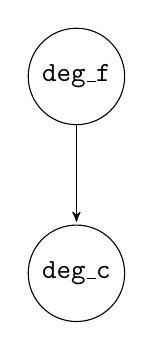
\begin{tikzpicture}[->,>=stealth',shorten >=1pt,auto,node distance=2.5cm]
\node[state] (1)                    {$\code{deg\_f}$};
\node[state] (2) [below of=1] {$\code{deg\_c}$};
\path[->] (1) edge node {} (2);
\end{tikzpicture}
\caption{The dependency tree for \emph{temp.rpl}}
\end{figure}

Suppose we have the following piece of code:
\begin{lstlisting}[title=\emph{link.rpl}]
...
int x = 10;
link( int y <- x + 2)
link ( int z <- y - 1)

link ( int q <- x - 3)
y = x + 7;
...
\end{lstlisting}

The dependency tree for \emph{link.rpl} is shown in Figure 2. As shown on line 3 through 4, there is a nested \code{link} statement within the initial \code{link} statement. This nesting is illustrated in the dependency tree by the addition of a new layer of nodes.

\begin{wrapfigure}{r}{0.3\textwidth}
\centering
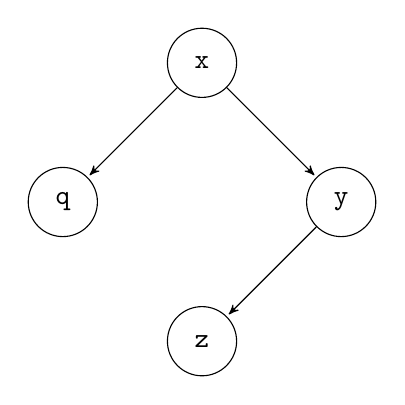
\begin{tikzpicture}[->,>=stealth',shorten >=1pt,auto,node distance=2.5cm]
\node[state] (x)                    {$\code{x}$};
\node[state] (y) [below right of=x] {$\code{y}$};
\node[state] (z) [below left of=y]  {$\code{z}$};
\node[state] (q) [below left of=x]  {$\code{q}$};
\path[->] (x) edge node {} (y);
\path[->] (x) edge node {} (q);
\path[->] (y) edge node {} (z);
\end{tikzpicture}
\caption{The dependency tree for \emph{link.rpl}}
\end{wrapfigure}

Let's walk through the program, starting on line 2, to see what's happening here.

\begin{description}
\item[Line 2] The variable \code{x} is initialized with the value of 10.
\item[Line 3] The variable \code{y} is initialized and linked to \code{x} through the statement \code{x + 2}; the value of \code{y} becomes 12. This creates the root node \code{x} and the child node \code{y} and connects them on the dependency tree.
\item[Line 4] The nested link statement initializes the integer variable \code{z} to the variable \code{y}; the value of \code{z} is 11. The node \code{z} is added to the dependency tree as a child of \code{y} and a link is made between them.

\item[Line 7] The variable \code{q} is initialized as an integer linked to \code{x}; the value of \code{q} is 7. The dependency graph creates the node \code{q} as a child of \code{x} and creates a link between them.
\item[Line 8] \code{y}'s value is changed to 17. This change will cause a cascade down to \code{z}, registering \code{z}'s new value as 16. However, the values of \code{x} and \code{q} remains at 10 and 7 respectively because both \code{variables} are not linked to \code{y}.
\end{description}

Moving back to the \code{temp.rpl} example; on line 11, when \code{deg\_f} is updated to the new value of 32, \code{deg\_c} is notified of the change and updates its value accordingly. This update causes the change in value seen on the fourth line of output. 

\code{link}s have the interesting property of being many-to-one; that is, we can have a variable link to a myriad of previously declared variables. When one of those parent variables is updated, the child will be updated accordingly. Again, the programmer must be careful in these cases not to create cycles in the dependency tree.

\section{Stream Readers}
\code{StreamReader}s are interesting consequences related to the \code{link} keyword within the Ripple language. The intuition behind their genesis is as follows: If the language is to be truly reactive, it would be necessary to have a construct that could handle live data coming from a variety of diverse sources. Thus, the \code{StreamReader} was born.

A \code{StreamReader} is fairly simple to implement within code itself, and has the ability to be extended for other types of media. Before we delve further into the implementation of \code{StreamReader}, let's look at a sample program.

A simple implementation of a \code{StreamReader} is a line counting program.

\begin{lstlisting}[title=\emph{count.rpl}]
import ``FileStreamReader'';

#**
* Reads in a file and prints out the line with the line number. 
**#

link void printLineNumber(int count, string line){
    count = count + 1;
    output(count, line, "\n");
}

void main(String[] args) {
    String filename = args[1];
    
    int count = 0;
    link (String line <- FileStreamReader(filename)) 
        printLineNumber(count, line);
}
\end{lstlisting}

Let's walk through the program to see how the \code{FileStreamReader} works.

\begin{description}
\item[Line 1] The \code{import} keyword tells the compiler that the program is using an external \code{StreamReader}. In this program, we are using the \code{FileStreamReader}, which provides a way to read through a file asynchronously line by line. This tool is an extension of of the generic \code{StreamReader} construct.
\item[Line 7] The \code{link} keyword before the function indicates that \code{printLineNumber()} will be provided to a link statement.
\item[Line 16] The \code{line} variable is initialized and linked to an  \code{FileStreamReader} which is created by providing it with a filename to open and iterate through.
\item[Line 17] The \code{printLineNumber()} function is called and passed the count function and line that was obtained from the \code{FileStreamReader}. All variables passed into functions provided to \code{link} statements are passed by value allowing them to be updated every time the \code{link} statement updates.
\end{description}

\begin{lstlisting}[title=\emph{temp3.rpl}]
import ``XMLStreamReader'';

#** 
 * Prints Fahrenheit-Celsius temperature based on stream 
 * from www.weather.gov 
 **#
FINAL float TEMP_CONV = 9 // 5;
void main(String[] args) {
    
    link(int deg_f <- (int) XMLStreamReader(``www.weather.gov'', 
                                            ``temp_farenheit'', 5))
        output(``Temperature in F: '', deg_f, ``\n'');
        
    link(int deg_c <- (deg_f - 32) * TEMP_CONV)
        output(``Temp in C: '', deg_c, ``\n'');
    
}
\end{lstlisting}

For simplicity's sake, we shall assume that the stream coming from \code{http://www.weather.gov} is of a well-formatted XML file, with the tag ``\code{farenheit}''. If we run the program after compilation, we have the following output.
\begin{flalign*}
\$ & \quad \textbf{rpl temp2.rpl} & \\
   & \quad \textbf{./temp2}       & \\
   & \code{Temperature in F: 27}  & \\
   & \code{Temperature in C: -3}  &
\end{flalign*}
The dependency tree for temp3 is shown in Figure 3.

Let's walk through the program to see how \code{XMLStreamReader} is implemented.

\begin{description}
\item[Line 1] The \code{import} keyword tells the compiler that the program is using an external library. In this program, we are importing \code{XMLStreamReader}, which contains a \code{StreamReader} to read streams of XML files. This construct is an extension of the generic \code{StreamReader} construct.
\item[Line 10] The \code{deg\_f} variable is initialized and linked to an  \code{XMLStreamReader} which is created by providing it with a URL, an XML tag to look for and a refresh time interval in seconds.
\item[Line 12] The \code{output} statement outputs the value of \code{deg\_f} to standard output. Since this function is provided to the link statement it is executed ever time the \code{XMLStreamReader} refreshes the feed.
\item[Lines 14 and 15] As above, when the \code{deg\_f} variable changes, the corresponding temperature in Celsius is calculated and printed.
\end{description}

\section{Final Statements}
Most modern programming languages have the concept of a read-only keyword that defines a value or construct at compile time and does not alter it at run time. Ripple is no exception. The keyword used for this read-only declaration is the \code{final} keyword followed by a construct declaration. 

Similar to C's macros and Java's \code{final} variables, these \code{final} variables must be declared and initialized at the top of the file and cannot change throughout the life of the program. Therefore, it is best to use these constructs for readability and maintainability of the code base. For example, in the source code for \emph{temp2.rpl}, the variable \code{TEMP\_CONV} is used to permanently store the conversion rate from Fahrenheit to Celsius.

\section{Conclusion}
This, hopefully, has given a general overview of the basics of Ripple. Unfortunately, this tutorial cannot give a full and in-depth discussion of the subtler intricacies of Ripple, especially when dealing with \code{link} statements and \code{StreamReaders}. However, we believe that we have provided enough tools and a general understanding of the core aspects of Ripple that you may begin experimenting and writing your own code, and we encourage you to go out and do so.

\end{document}